\documentclass[]{book}
\usepackage{lmodern}
\usepackage{amssymb,amsmath}
\usepackage{ifxetex,ifluatex}
\usepackage{fixltx2e} % provides \textsubscript
\ifnum 0\ifxetex 1\fi\ifluatex 1\fi=0 % if pdftex
  \usepackage[T1]{fontenc}
  \usepackage[utf8]{inputenc}
\else % if luatex or xelatex
  \ifxetex
    \usepackage{mathspec}
  \else
    \usepackage{fontspec}
  \fi
  \defaultfontfeatures{Ligatures=TeX,Scale=MatchLowercase}
\fi
% use upquote if available, for straight quotes in verbatim environments
\IfFileExists{upquote.sty}{\usepackage{upquote}}{}
% use microtype if available
\IfFileExists{microtype.sty}{%
\usepackage{microtype}
\UseMicrotypeSet[protrusion]{basicmath} % disable protrusion for tt fonts
}{}
\usepackage[margin=1in]{geometry}
\usepackage{hyperref}
\hypersetup{unicode=true,
            pdftitle={Do not use averages on Likert scale data},
            pdfauthor={Dwight Barry},
            pdfborder={0 0 0},
            breaklinks=true}
\urlstyle{same}  % don't use monospace font for urls
\usepackage{natbib}
\bibliographystyle{plainnat}
\usepackage{longtable,booktabs}
\usepackage{graphicx,grffile}
\makeatletter
\def\maxwidth{\ifdim\Gin@nat@width>\linewidth\linewidth\else\Gin@nat@width\fi}
\def\maxheight{\ifdim\Gin@nat@height>\textheight\textheight\else\Gin@nat@height\fi}
\makeatother
% Scale images if necessary, so that they will not overflow the page
% margins by default, and it is still possible to overwrite the defaults
% using explicit options in \includegraphics[width, height, ...]{}
\setkeys{Gin}{width=\maxwidth,height=\maxheight,keepaspectratio}
\IfFileExists{parskip.sty}{%
\usepackage{parskip}
}{% else
\setlength{\parindent}{0pt}
\setlength{\parskip}{6pt plus 2pt minus 1pt}
}
\setlength{\emergencystretch}{3em}  % prevent overfull lines
\providecommand{\tightlist}{%
  \setlength{\itemsep}{0pt}\setlength{\parskip}{0pt}}
\setcounter{secnumdepth}{5}
% Redefines (sub)paragraphs to behave more like sections
\ifx\paragraph\undefined\else
\let\oldparagraph\paragraph
\renewcommand{\paragraph}[1]{\oldparagraph{#1}\mbox{}}
\fi
\ifx\subparagraph\undefined\else
\let\oldsubparagraph\subparagraph
\renewcommand{\subparagraph}[1]{\oldsubparagraph{#1}\mbox{}}
\fi

%%% Use protect on footnotes to avoid problems with footnotes in titles
\let\rmarkdownfootnote\footnote%
\def\footnote{\protect\rmarkdownfootnote}

%%% Change title format to be more compact
\usepackage{titling}

% Create subtitle command for use in maketitle
\newcommand{\subtitle}[1]{
  \posttitle{
    \begin{center}\large#1\end{center}
    }
}

\setlength{\droptitle}{-2em}
  \title{Do not use averages on Likert scale data}
  \pretitle{\vspace{\droptitle}\centering\huge}
  \posttitle{\par}
  \author{Dwight Barry}
  \preauthor{\centering\large\emph}
  \postauthor{\par}
  \predate{\centering\large\emph}
  \postdate{\par}
  \date{2017-01-02}

\usepackage{booktabs}

\begin{document}
\maketitle

{
\setcounter{tocdepth}{1}
\tableofcontents
}
\chapter{Summary}\label{summary}

\begin{itemize}
\item
  Likert and similar ordinal-level scales have a variety of uses,
  particularly within surveys. They also occur in clinical care, for
  example, in the use of pain scores.
\item
  When evaluated improperly---particularly through the use of
  averages---the results can be strikingly misleading. Obviously,
  misleading results could drive or promote action where none is
  warranted, and vice versa.
\item
  In nearly all cases, not only is it mathematically wrong,
  \textbf{taking the average of a Likert-scale variable will \emph{not}
  provide useful answers} to the questions end-users can use to make
  actionable decisions. In essence, the use of averages cannot account
  for the importance of capturing and understanding variabililty.
  Analysts should strive to avoid their use in any reporting solution or
  analytic product that uses ordinal-scale data.
\item
  Better ways to represent ordinal-value results include histograms of
  the values themselves, the use of well-supported ``top-box''-type
  proportions, and/or bar charts of percentage by score or score
  category (e.g., favorable/neutral/unfavorable).
\item
  ``Statistical significance'' on changes or differences between
  response groups' medians or distribution shift can be assessed through
  non-parametric frequentist tests (e.g., permutation,
  Mann-Whitney-Wilcoxon), Information Theory, or Bayesian analysis.
  \emph{t}-tests should never be used on Likert scales because ordinal
  data does not meet the assumptions of a \emph{t}-test (and when using
  frequentist tools, one must \emph{also} account for multiple testing
  to reduce the chance of false positives).
\item
  A good way to remember not to use means on Likert scale data is to
  think: The average of \emph{Agree} and \emph{Strongly Agree} is
  \textbf{not} \emph{Agree-And-A-Half}.
\end{itemize}

\emph{Note: all of the data in this document is fake, created
specifically to illustrate particular points.}

\chapter{A simple example}\label{a-simple-example}

Take a simple example where a group of 6 people people take the same
survey for 4 years, and the mean results for an important question, such
as ``my team works well together'', are as follows:

Taking the mean of these results gives you this:

\begin{longtable}[]{@{}cccc@{}}
\toprule
Year 1 & Year 2 & Year 3 & Year 4\tabularnewline
\midrule
\endhead
4.17 & 4.33 & 4.33 & 4.33\tabularnewline
\bottomrule
\end{longtable}

From these values, one might conclude that there is an improvement from
year 1 to year 2, and no change year-over-year after year 2.

The values that created the above results are as follows:

\begin{tabular}{l|r|r|r|r}
\hline
Individual & Year 1 & Year 2 & Year 3 & Year 4\\
\hline
A & 5 & 2 & 3 & 1\\
\hline
B & 4 & 5 & 5 & 5\\
\hline
C & 4 & 5 & 5 & 5\\
\hline
D & 4 & 5 & 5 & 5\\
\hline
E & 4 & 5 & 5 & 5\\
\hline
F & 4 & 4 & 3 & 5\\
\hline
\end{tabular}

You might already see how management decisions would be made differently
based on whether one had just the means or had the complete data.

However, in the latter case, you risk reducing or eliminating anonymity,
which is essential to get respondents to answer truthfully (not to
mention being unethical). Further, poring over tables of answers for
many people for long surveys makes that approach practically infeasible.
Visualizing the results in ways that capture a more complete story
provides an answer to both issues, as well as providing decision-makers
with truly actionable information.

\chapter{Visualization}\label{visualization}

\section{Histograms}\label{histograms}

Histograms of the actual score values are the best way to visualize
Likert data---they have two real axes, showing counts by score value or
category, so you can parse the visual and understand the results very
quickly. Using the same data as above, you can instantly see that the
``improvement'' in year 2 was perhaps not an improvement after all:
while most respondents appear to be satisfied above what they thought in
year 1, one respondent may be at risk of leaving.

\emph{Figure 1. Histogram of example Likert scale data.}

\begin{center}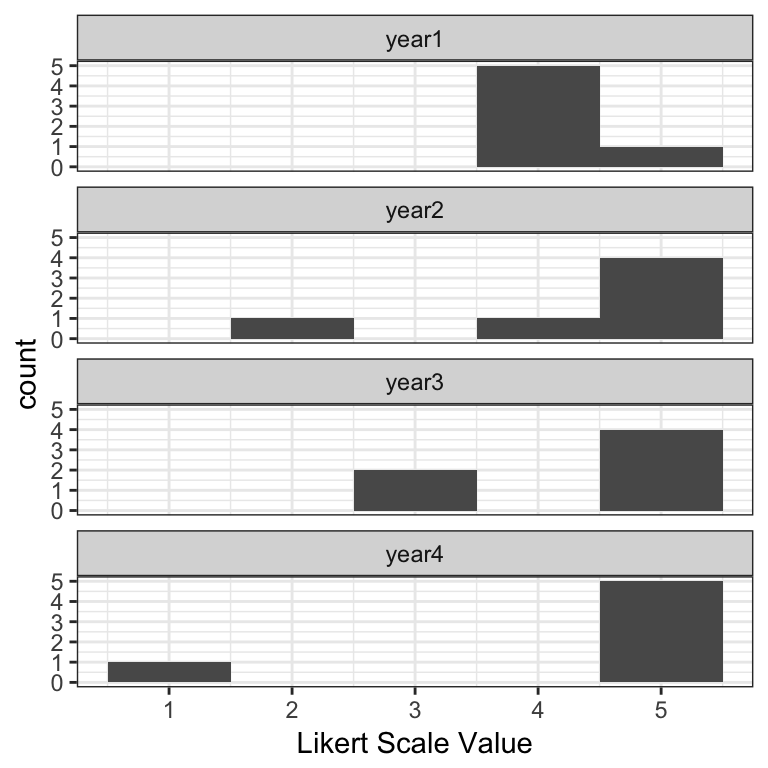
\includegraphics{bookdown-demo_files/figure-latex/histos-1} \end{center}

\section{Likert charts}\label{likert-charts}

The main disadvantage of histograms is space; Likert charts---which are
in essence just stacked bar charts---are far more compact. The
disadvantage is that it takes slightly longer for a user to parse them,
but when faced with lots of questions or groupings, they tend to be a
better option.

There are two kinds of Likert charts---those that use a center line for
a point of reference, and those that do not, in which case they are
simply percentage bar charts for individual questions or are mosaic
plots when comparing groupings. In the graphs below, each score value
has its own color, and each score category---e.g., unfavorable is 1-2,
neutral is 3, and favorable is 4-5 on a 5-point scale---is summarized by
a percentage value at the left, middle/interior, and right sides of the
bar, respectively.

\emph{Figure 2. Centered Likert chart.}

\begin{center}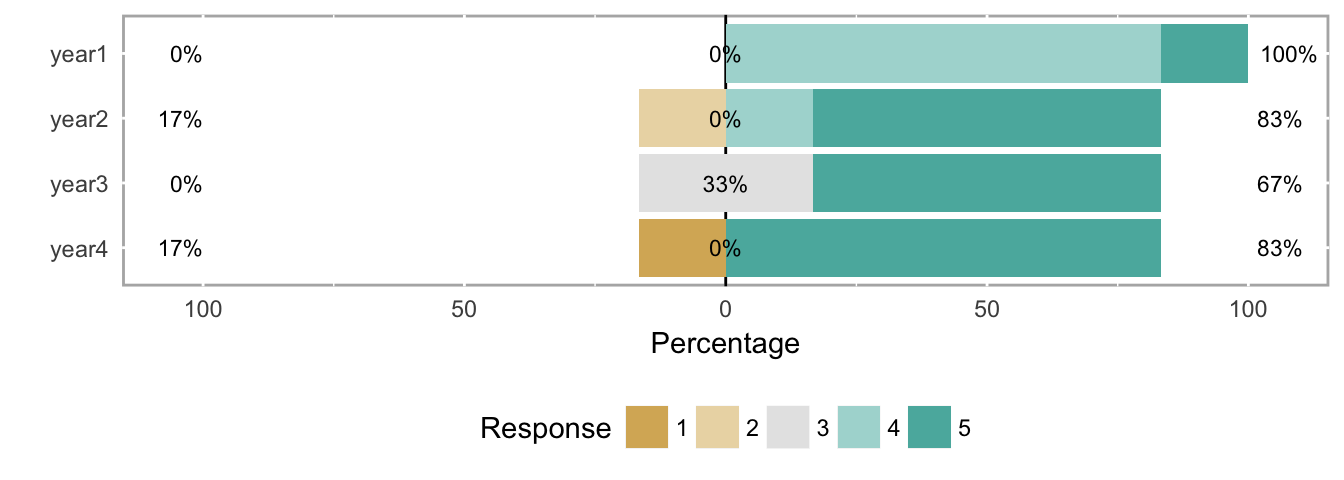
\includegraphics{bookdown-demo_files/figure-latex/ex_1_likert-1} \end{center}

\emph{Figure 3. Uncentered Likert chart (aka percent bar chart).}

\begin{center}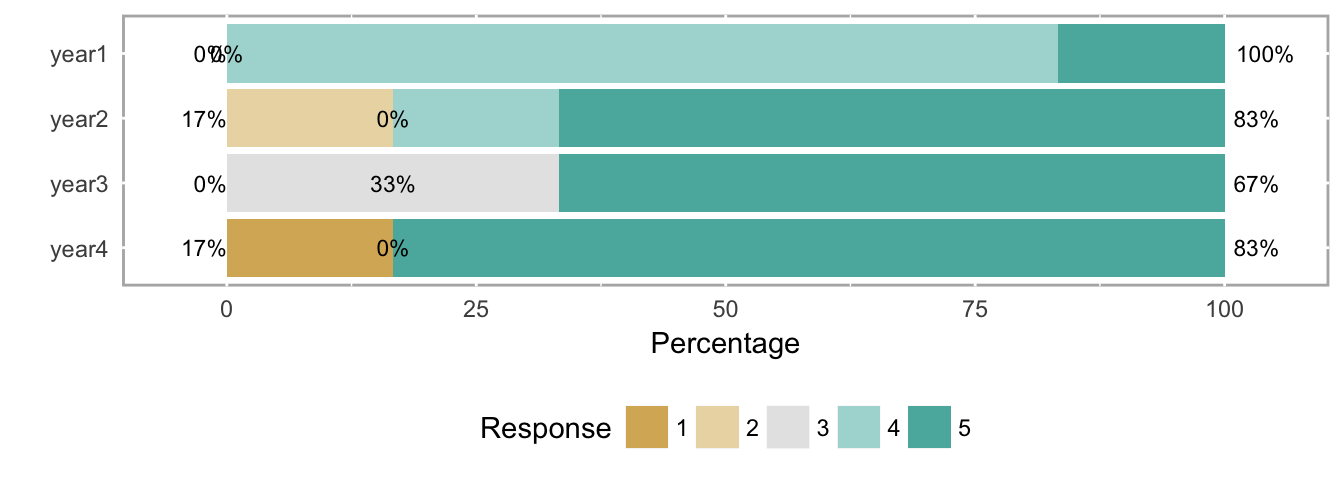
\includegraphics{bookdown-demo_files/figure-latex/ex_1_likert_percent-1} \end{center}

Neither Likert chart type is as clear as the histogram at making the
results immediately understandable, but again, histograms take more
space, and busy decision makers often need to see the forest (all the
questions) at the expense of some trees (each question). In this case,
analysts might use the histograms to explore potentially important
results themselves, and then use Likert charts in a report with some
strategically-placed text highlighting important patterns they found
with the histograms.

\section{Other ordinal-scale
visualizations}\label{other-ordinal-scale-visualizations}

\subsection{Likert chart with response count
histograms}\label{likert-chart-with-response-count-histograms}

\emph{Figure 6. A Likert chart for two different questions (e.g., as
within a single year's survey), with a count histogram to show number of
responses and non-answers for each question.}

\begin{center}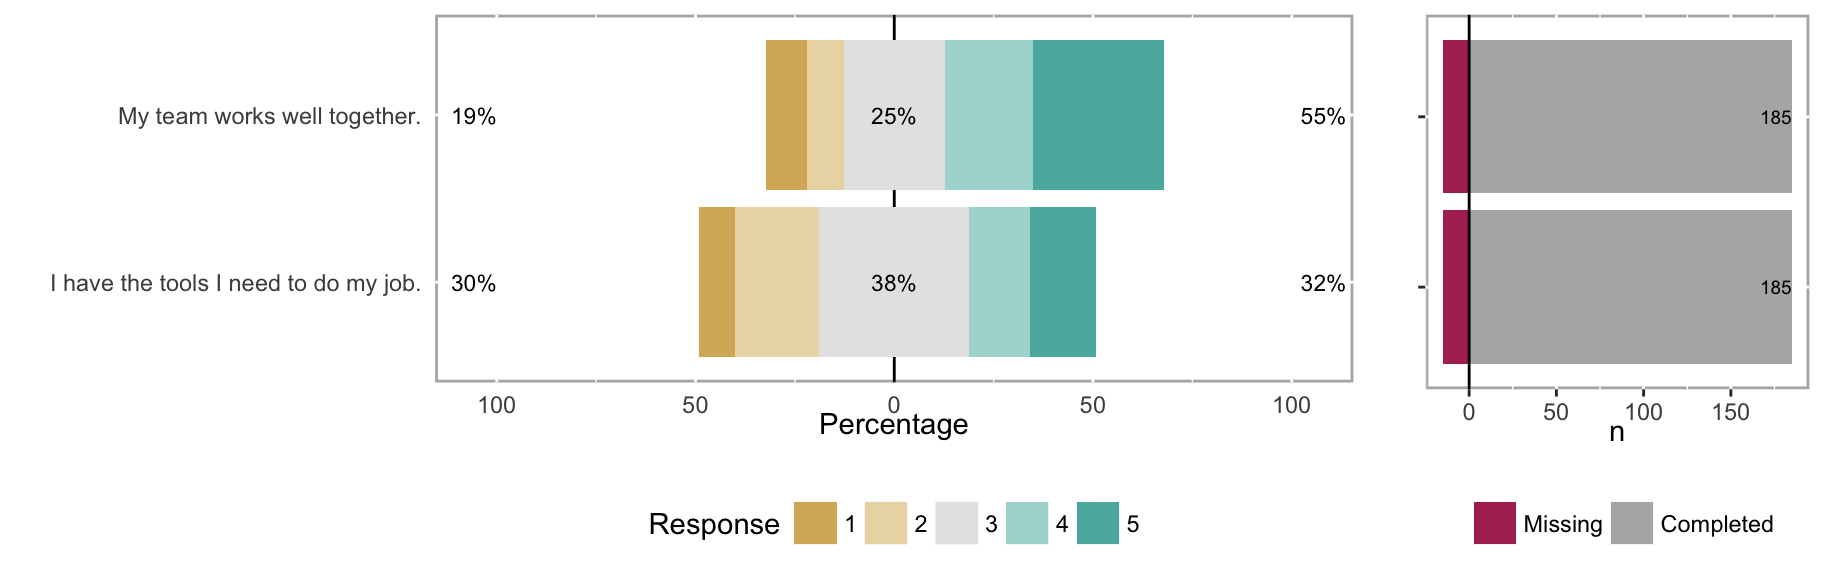
\includegraphics{bookdown-demo_files/figure-latex/likert_viz1-1} \end{center}

~

\subsection{Uncentered Likert chart for multiple
questions}\label{uncentered-likert-chart-for-multiple-questions}

\emph{Figure 7. An uncentered Likert chart for two different questions.}

\begin{center}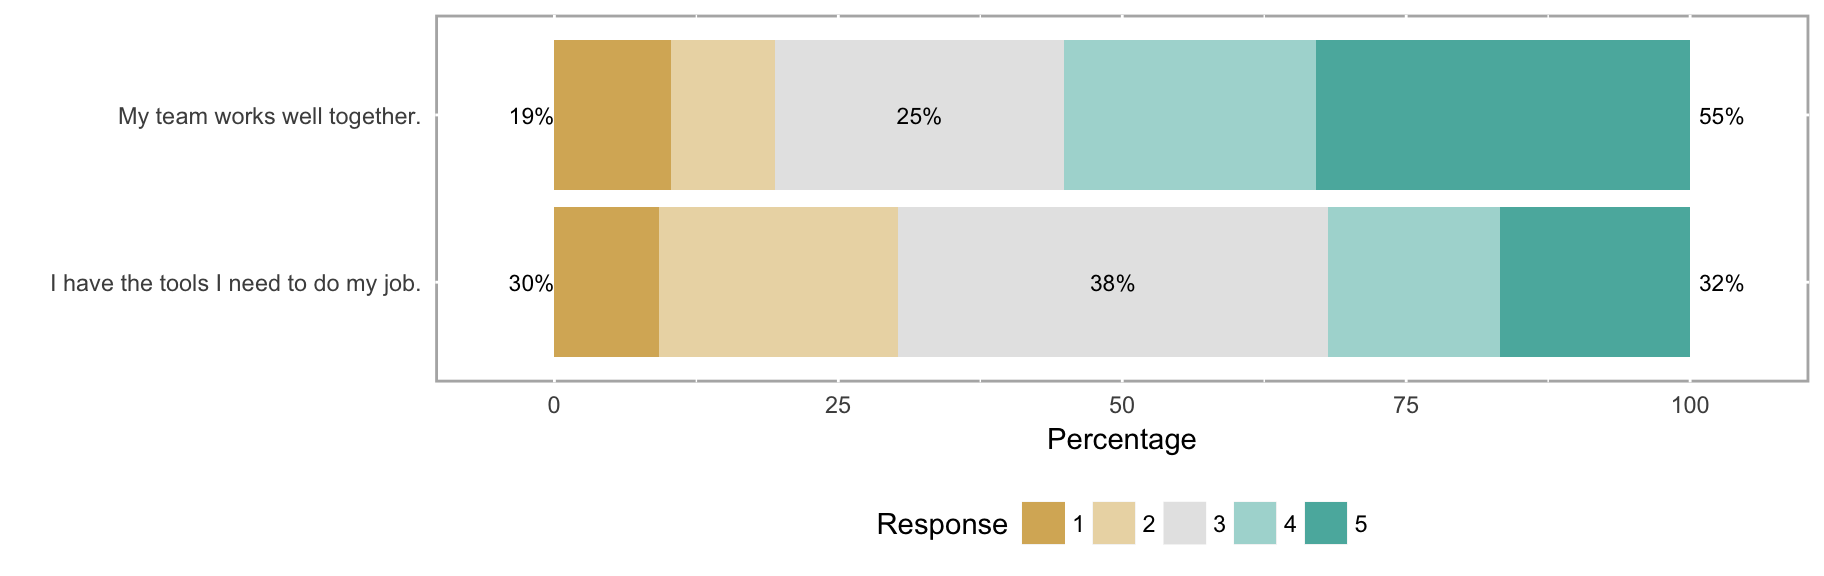
\includegraphics{bookdown-demo_files/figure-latex/likert_viz2-1} \end{center}

~

\subsection{Heatmap}\label{heatmap}

\emph{Figure 8. A heatmap of the response frequency for two different
questions. While the use of means and SDs is inappropriate, this
particular example directly illustrates why those values don't capture
the response patterns in the data.}

\begin{center}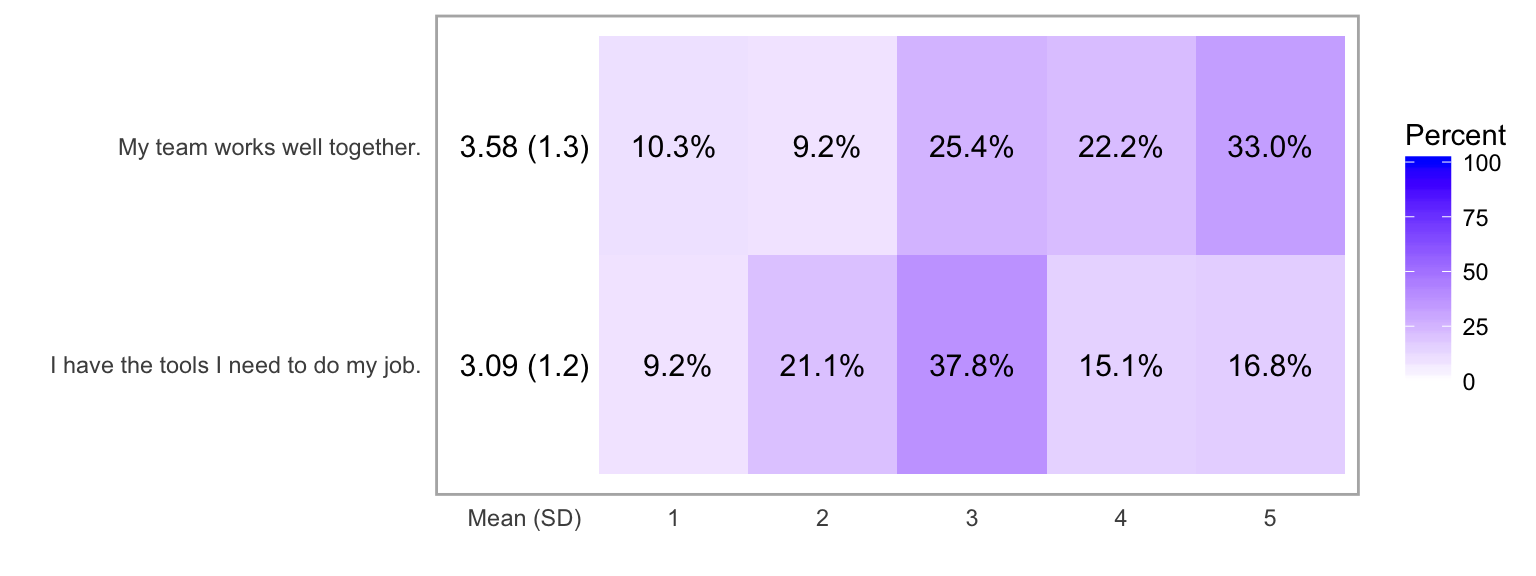
\includegraphics{bookdown-demo_files/figure-latex/likert_viz3-1} \end{center}

~

\subsection{Likert chart with
subgroups}\label{likert-chart-with-subgroups}

\emph{Figure 9. Subgroups can sometimes reveal patterns not seen in
aggregate data. For example, compare the overall results for ``My team
works well together'' in Figure 5 (above) with the responses from the
subgroups of MDs and RNs (below, bottom panel).}

\begin{center}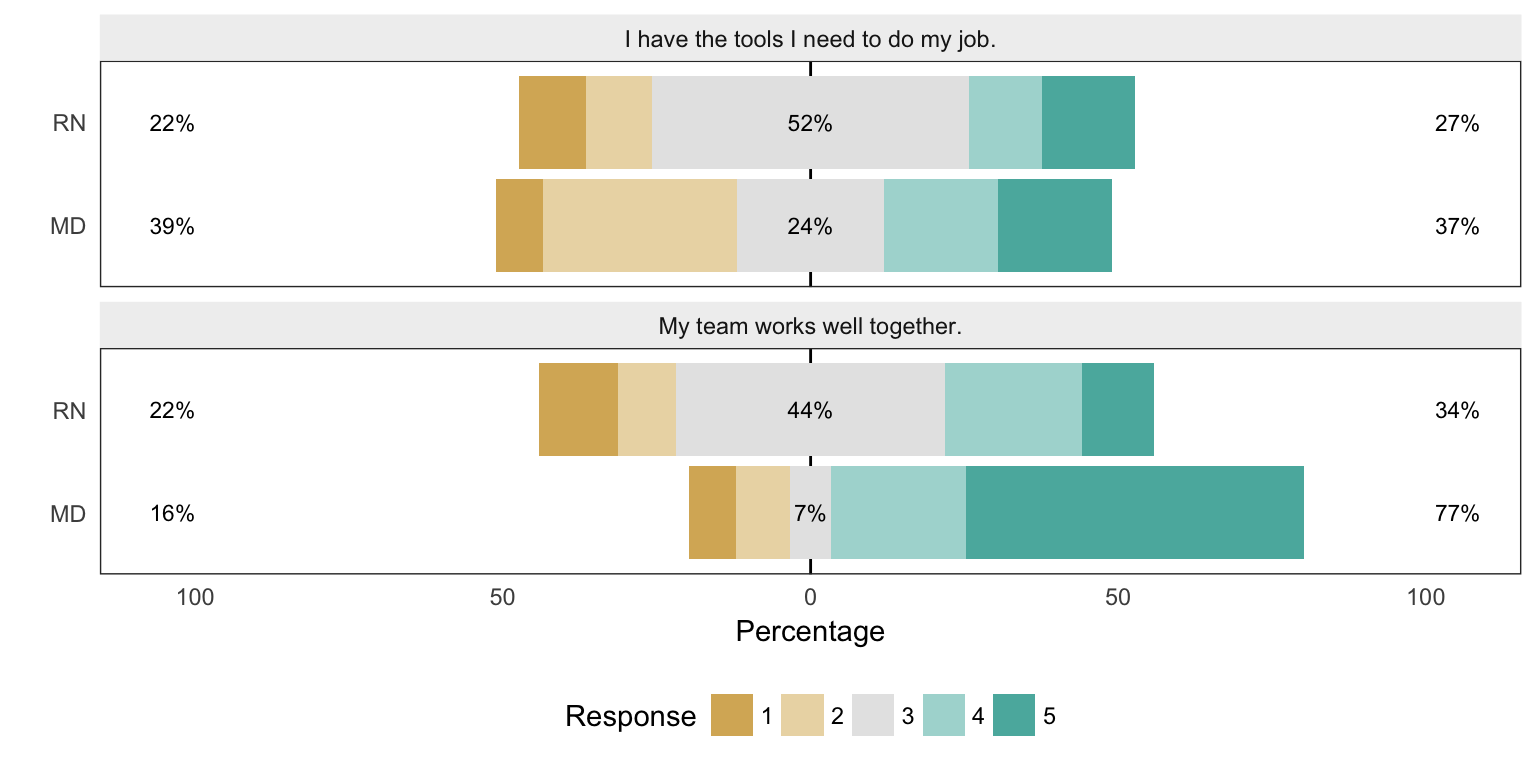
\includegraphics{bookdown-demo_files/figure-latex/likert_viz4-1} \end{center}

~

\subsection{Density histograms}\label{density-histograms}

\emph{Figure 10. Density plots for the same data shown in Figure 8,
above. While using a density plot on ordinal data is also statistically
inappropriate, it can be a useful tool for an analyst. Bar histograms
are difficult to overlay subgroups or different years for a direct
comparsion, so must be separated into facets instead (e.g., Figure 1,
above). Density plots are easier to overlay to show these comparisons,
so while not appropriate for a report, they can be useful tools for an
analyst during the exploration phase.}

\begin{center}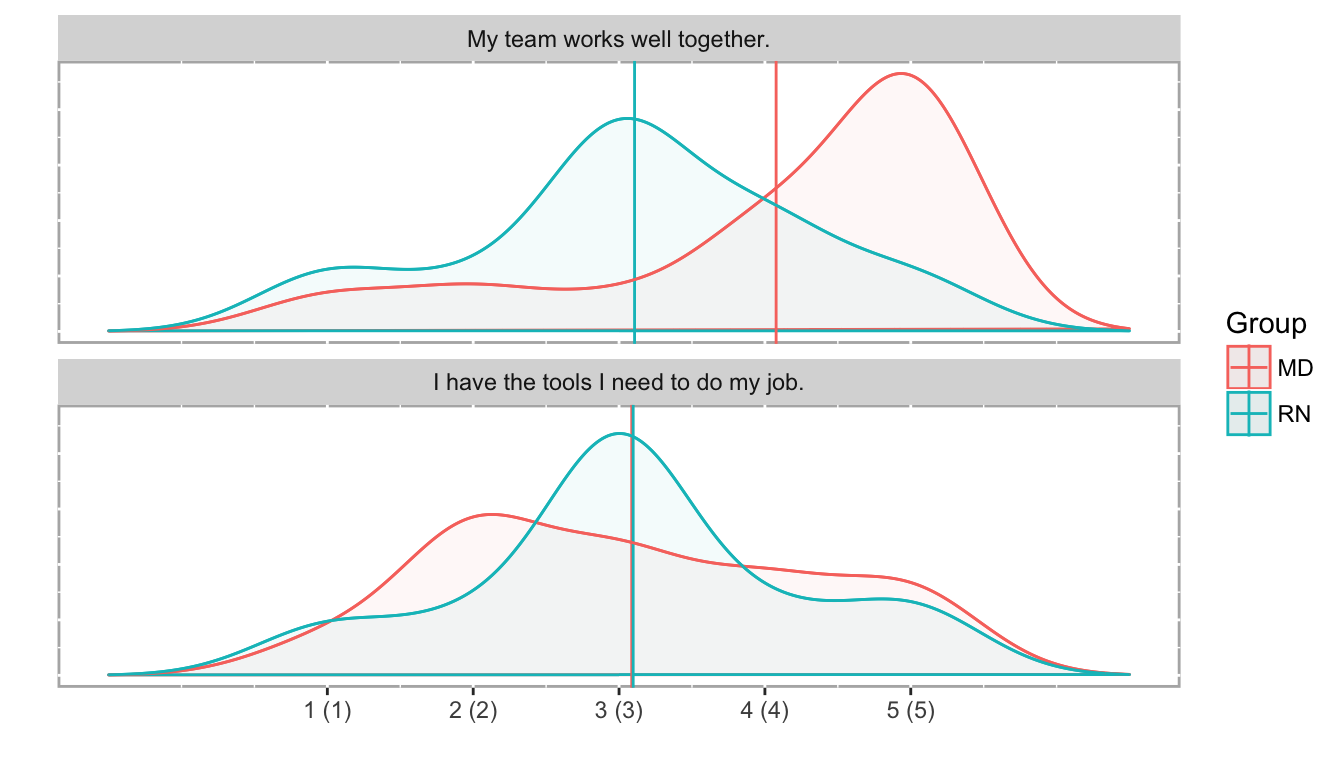
\includegraphics{bookdown-demo_files/figure-latex/likert_viz5-1} \end{center}

\chapter{Tips and Tricks}\label{tips-and-tricks}

\section{\texorpdfstring{\emph{Neutral} scores
matter}{Neutral scores matter}}\label{neutral-scores-matter}

You might have noticed in some surveys that there is often no
``neutral'' or ``undecided'' category included in the middle of the
scale, e.g., what's usually a 3 on a 5-point Likert scale. Sometimes it
is placed at the end of the scale, and sometimes it is eliminated
entirely. The reason for this is that those terms can sometimes be
interpreted in a variety of ways; for example, with a question such as
``My pay is fair compared with other companies'', a \emph{Neutral}
response could indicate ``I'm neutral on this'', ``yes, I guess so'',
``I don't know'', ``it's neither fair nor unfair'', ``I don't want to
answer'', ``I'm not sure what `fair' means'', and any number of ideas
that don't necessarily indicate a true neutral opinion.

When a question has a response option where this type of ambiguity
exists, a mean value will tend toward the that option because of this
bias, unless of course the mean is already at that value. However, when
\emph{Neutral} is marked as 3, and when valid responses tend towards 4s
and 5s, these ambiguous responses will drag down the average (and vice
versa for responses heavy with 1s and 2s). Of course, you shouldn't use
means anyway, as we've seen above, but many reports do---so
understanding this effect is important toward interpreting the results
in a useful way.

Use of a median is somewhat resistant to this problem, though you still
won't know whether the middle values are valid responses or accidents of
interpretation.

When you see an ``undecided'' or ``N/A'' response placed at the end of
the scale or missing entirely, it is usually (but not always!) a sign
that the survey creator understands this problem.

Sometimes, of course, \emph{Neutral} can be a completely reasonable and
unambiguous response to a question. Context matters; while it's easiest
for survey creators and scanning software to use the same scale for
large numbers of questions, it is important that the analyst understand
the extent to which \emph{Neutral} and similar types of responses are a
valid part of the measurement scale for each question.

\section{How many respondents are
enough?}\label{how-many-respondents-are-enough}

It's common to think: ``We surveyed everyone in this department,
therefore the results we see must be correct.'' However, how people
responded to surveys depends on many factors---such as mood the date the
survey is taken, recent events in life and in work, changes in
organizational structure, and any number of other factors---and many
internal surveys are given only once a year. Thus, survey results are
really a \emph{sample} of attitudes and opinions, subject to random
events and natural fluctuations.

Typical practice at some companies is to expose summary results for
groups with six or more people. While this helps preserve some
anonymity, it does not include enough responses to ensure the overall
response is stable. Comparisons over time or across groups that are not
based on stable results can lead to conclusions about differences that
may or may not reflect reality.

In this context, \emph{stable} means that the data accurately represent
true changes (or lack of change) in the question at hand. It's basically
impossible to distinguish natural variation from real change when you
have small numbers of respondents. As a result, the National Center for
Health Statistics, for example, does not publish results with less than
20 distinct cases or responses.

The relative standard error (RSE) is the metric used to evaluate whether
you have enough values for the results to be stable. The standard error
is an estimate of the likely difference between the results and the true
value (which in surveys, even of complete populations, can't be known
exactly due to the reasons mentioned above). The \emph{relative}
standard error is the standard error expressed as a percent of the
measure or number of responses, which is a constant function:
\(\frac{1}{\sqrt{responses}} * 100\). This function can be seen in the
graph on the next page.

Generally, you want RSE values less than 20-25\% to have some confidence
that your results are stable.

\emph{Figure 4. The RSE-response count function. The RSE associated with
the use of 6 responses is marked with dark red, and the response count
associated with an RSE of 25\% is marked with dark blue.}

\begin{center}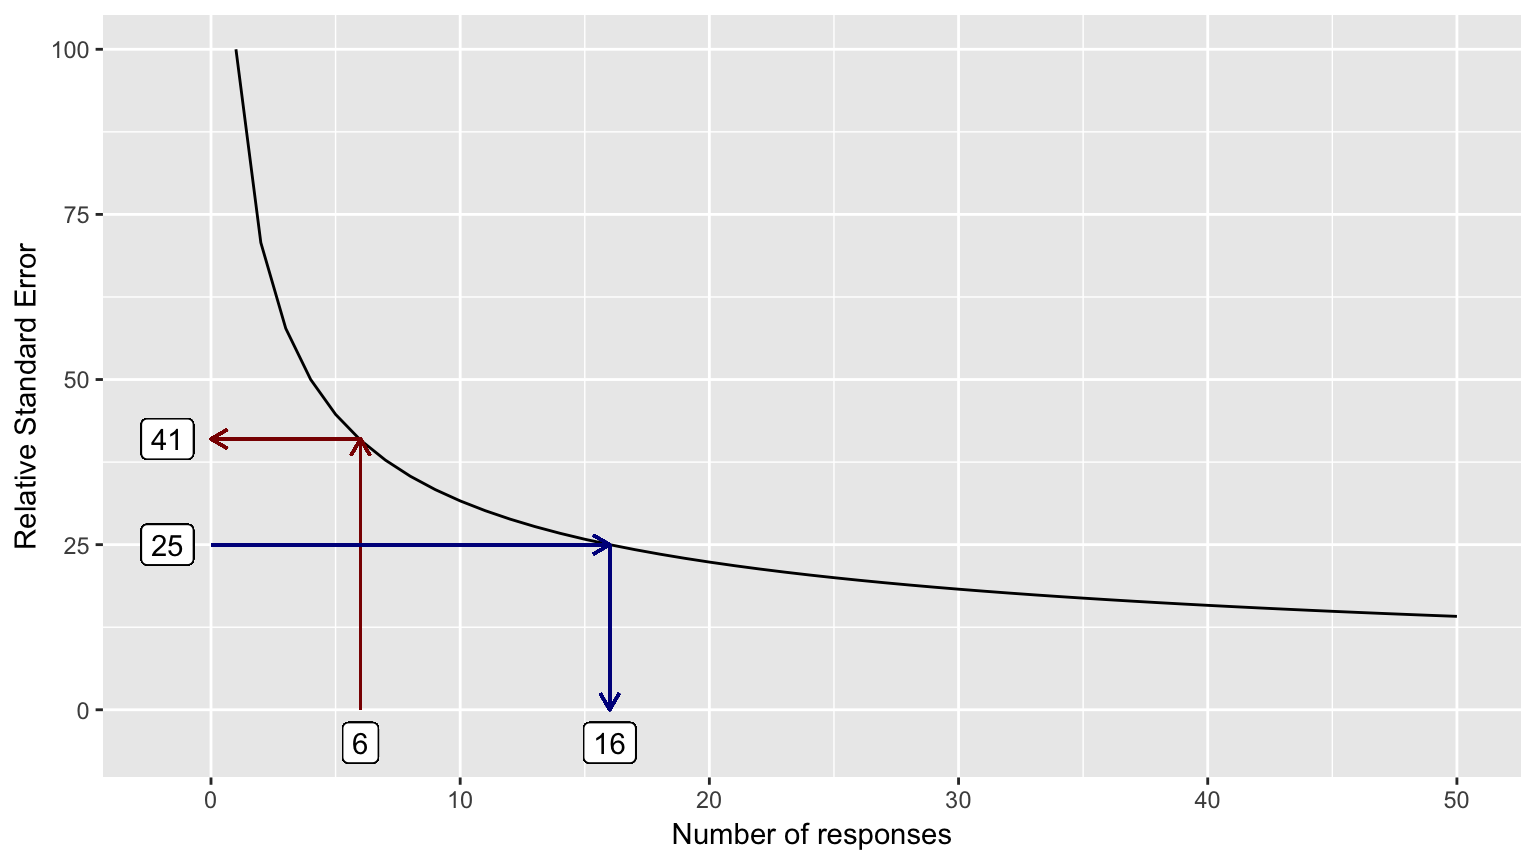
\includegraphics{bookdown-demo_files/figure-latex/rse-1} \end{center}

\chapter{\texorpdfstring{Is there a \emph{significant}
difference?}{Is there a significant difference?}}\label{is-there-a-significant-difference}

Many decision-makers want to know if a result is ``significantly
different'' from, say, the same response from a previous time period, or
between a couple of subgroups in the same response. Unfortunately, this
is mostly useless, for two reasons.

First, acting as if Likert or other ordinal scales are continuous level
data leads to many problems of interpretation (see the
\protect\hyperlink{Appendix}{\emph{Appendix}} for a summary table of
measurement scales and appropriate statistics). There has been
controversy over this distinction for many decades; however, a great way
to understand the conceptual problem is to realize that the mean of
\emph{Agree} and \emph{Strongly Agree} is \textbf{not}
\emph{Agree-And-A-Half}---it just makes no sense.

A subsequent argument might be that, no, it's not conceptually accurate,
but it provides a sense for directional changes. However, such results
still run into problems of interpretation: if you go from 4.16 to 4.33,
have you gone from \emph{Agree.16} to \emph{Agree.33}? What does such an
``improvement'' mean, in practical terms? All you can accurately say is
that both values are most consistent with an \emph{Agree} opinion.

Specifically in the medicine/healthcare context,
\href{https://www.ncbi.nlm.nih.gov/pubmed/8883724}{Kuzon et al.} state
that the use of parametric statistics on ordinal data (such calculating
a mean or using a \emph{t}-test) is the first of ``The seven deadly sins
of statistical analysis''. Don't ``sin'' and you don't have to worry
about whether your results are illegitmate.

There are a few ways around this: 1) use medians or other quantiles and
test for differences in those statistics (these differences are best
assessed via bootstrap or permutation testing), 2) test whether the
distribution has shifted (Mann-Whitney-Wilcoxon test), or 3) use more
advanced techniques such as multinomial or proportional-odds regression
(see the \protect\hyperlink{Advanced}{\emph{Advanced}} section). These
options are the more statistically-correct ways to do it (as opposed a
\emph{t}-test).

So, using the simple example above, we might want to know whether the
median is statistically different between year 1 (Median = 4) and year 2
(Median = 5). Running a
\href{https://en.wikipedia.org/wiki/Resampling_(statistics)\#Permutation_tests}{permutation
test} gives us the following results:

\begin{verbatim}
>  
>   Exact Two-Sample Fisher-Pitman Permutation Test
>  
>  data:  value by variable (year1, year2)
>  Z = -0.33333, p-value = 1
>  alternative hypothesis: true mu is not equal to 0
\end{verbatim}

While our effect size is ``1''---more accurately, \emph{Agree} to
\emph{Strongly Agree}---the \emph{p}-value of the test is very large
(basically 1), so we cannot say that this difference is ``statistically
significant''.

We could also ask, ``has the distribution shifted?'', which would
involve using the
\href{https://en.wikipedia.org/wiki/Mann\%E2\%80\%93Whitney_U_test}{Mann-Whitney-Wilcoxon
test}:

\begin{verbatim}
>  
>   Wilcoxon rank sum test with continuity correction
>  
>  data:  value by variable
>  W = 11.5, p-value = 0.285
>  alternative hypothesis: true location shift is not equal to 0
\end{verbatim}

The \emph{p}-value is non-significant, so the difference between year 1
and year 2 can't be assumed to be a statistically significant change.

Looking at the raw data or graphs seen earlier, a decision-maker might
be justified in wanting to act, but the analysis suggests that the
difference is not statistically significant.

This leads us to the second problem with using \emph{p}-values for
determining whether a statistically-significant difference has occurred:
sample size.

\emph{p}-values are directly dependent on sample size. If your sample is
large enough, you are guaranteed to have a small \emph{p}-value. If your
sample is small, whether or not you get a significant \emph{p}-value
depends on the scale of difference between the groups, i.e., the effect
size.

For example, consider the following examples evaluating the number of
people who answer \emph{Agree} or \emph{Strongly Agree} (the
``favorable'' score group) to a question:

\begin{longtable}[]{@{}lrrcc@{}}
\toprule
Example & Favorable & Total Answers & Effect size &
\emph{p}-value\tabularnewline
\midrule
\endhead
1 & 15 & 20 & 75\% & 0.04\tabularnewline
2 & 114 & 200 & 57\% & 0.04\tabularnewline
3 & 1,046 & 2,000 & 52\% & 0.04\tabularnewline
4 & 1,001,450 & 2,000,000 & 50\% & 0.04\tabularnewline
\bottomrule
\end{longtable}

With 15 of 20 people selecting a favorable value on the Likert scale, we
have an effect size of 75\%, which is certainly an effect worth taking
seriously. That value is also a statistically significant difference
(\emph{p} \textless{} 0.05), which supports the idea that the majority
has a favorable opinion. With a couple of thousand responses (example
3), we again have a statistically significant difference, but the effect
size is now only 52\%, close enough to even-preference as to be
\emph{practically} the same. In medical terms, we might think of this as
statistically significant but clinically irrelevant.

For these
reasons---\href{http://www.tandfonline.com/doi/full/10.1080/00031305.2016.1154108}{and
many others outside the scope of these guidelines}---statisticians are
moving away from the use of \emph{p}-values. In frequentist statistics,
these are being replaced by the use of effect sizes and confidence
intervals (CIs); these provide information on both on the precision of
the estimated difference, as well as whether the difference can be
considered statistically distinct. If the CI includes 0, the difference
is not-significant. Regardless of the location of 0, the width of the CI
tells you how precise your estimate is.

\begin{verbatim}
>  Difference in medians is 1.
\end{verbatim}

\begin{verbatim}
>  BOOTSTRAP CONFIDENCE INTERVAL CALCULATIONS
>  Based on 1000 bootstrap replicates
>  
>  CALL : 
>  boot.ci(boot.out = median_diff, type = "perc")
>  
>  Intervals : 
>  Level     Percentile     
>  95%   (-1,  1 )  
>  Calculations and Intervals on Original Scale
\end{verbatim}

Here, we see that the effect size is a difference in medians of 1, but
the confidence interval on that effect size goes from -1 to +1, i.e.~is
consistent with any score difference between \emph{Neutral} and
\emph{Strongly Agree}. Since that CI includes 0, we can't say that the
change from median of \emph{Agree} to a median of \emph{Strongly Agree}
is statistically different, though again, sample size matters---one
would probably like to try to intervene based on the one respondent who
dropped down to 2 (\emph{Disagree}) anyway.

\hypertarget{Advanced}{\chapter{Advanced analytics for ordinal scaled
variables}\label{Advanced}}

\section{\texorpdfstring{\(\chi^2\)
test}{\textbackslash{}chi\^{}2 test}}\label{chi2-test}

While Mann-Whitney-Wilcoxon (sometimes known as the Mann-Whitney
\emph{U}-test) is the test most often used with differences between
ordinal distributions, there are other options that can tell you whether
a measured difference between groups is statistical different.

The old stand-by in this case is the \(\chi^2\) test, which is often
best visualized with a mosaic plot.

\emph{Figure 11. Chi-square test and mosaic plot between Employee Type
and responses to the ``My team works well together'' question.}

\begin{center}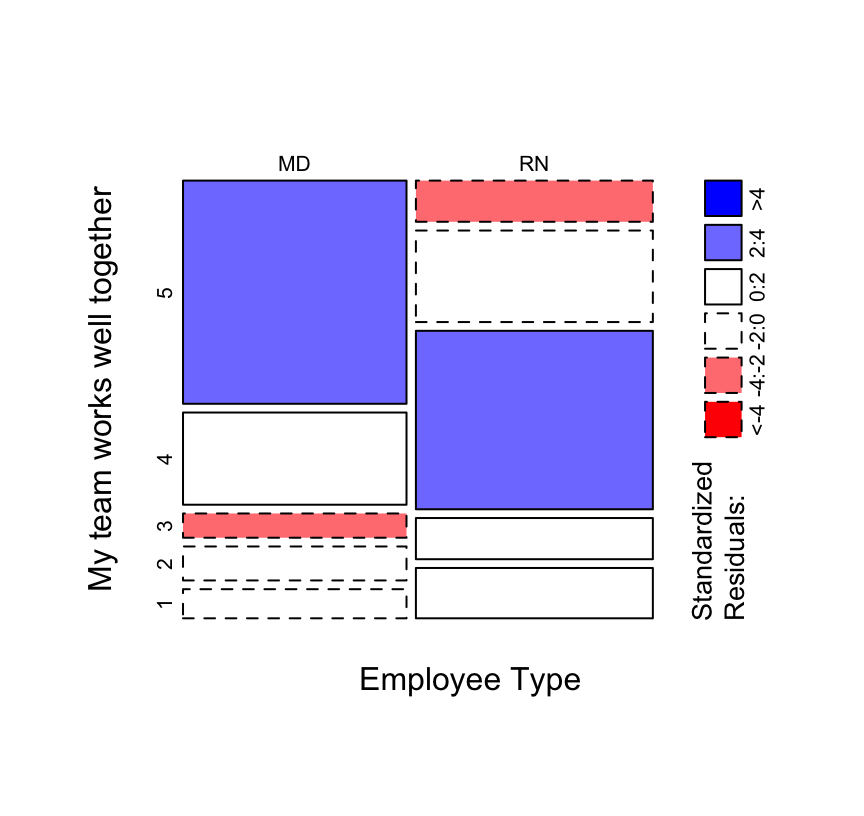
\includegraphics{bookdown-demo_files/figure-latex/mosaicplot-1} \end{center}

\begin{verbatim}
>  
>   Pearson's Chi-squared test with simulated p-value (based on 2000
>   replicates)
>  
>  data:  both2_tab
>  X-squared = 52.809, df = NA, p-value = 0.0004998
\end{verbatim}

~

\section{Multinomial regression}\label{multinomial-regression}

The multinomial regression model is a more powerful (and more modern)
version of the \(\chi^2\) test.

~

\emph{Figure 12. Multinomial regression between Employee Type and
responses to the ``My team works well together'' question, with
information-theoretic table for multi-model inference.}

\begin{center}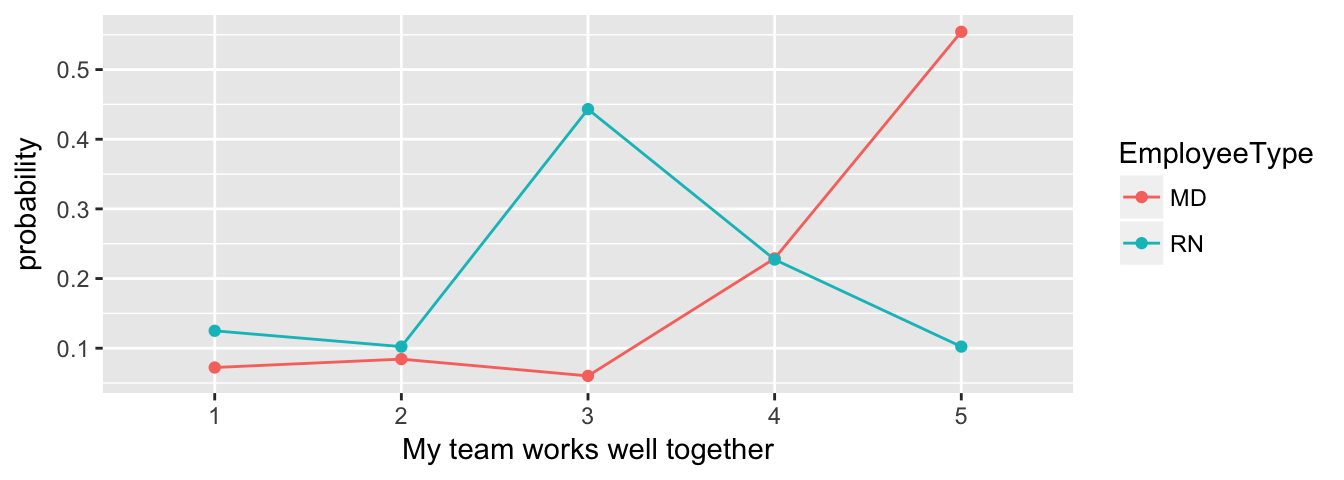
\includegraphics{bookdown-demo_files/figure-latex/multnom_plot-1} \end{center}

\begin{tabular}{l|r|r|r|r|r|r|r}
\hline
Modnames & K & AICc & Delta\_AICc & ModelLik & AICcWt & LL & Cum.Wt\\
\hline
Employee Type & 8 & 472.0249 & 0.00000 & 1 & 1 & -227.5680 & 1\\
\hline
Null Model & 4 & 522.0647 & 50.03976 & 0 & 0 & -256.9118 & 1\\
\hline
\end{tabular}

\section{Proportional-odds
regression}\label{proportional-odds-regression}

If you can meet the assumptions, the proportional-odds regression is
more powerful than the multinomial model, as it can take into account
the ordered nature of the ordinal scale.

\emph{Figure 13. Proportional odds logistic regression between Employee
Type and responses to the ``My team works well together'' question, with
information-theoretic table for multi-model inference.}

\begin{center}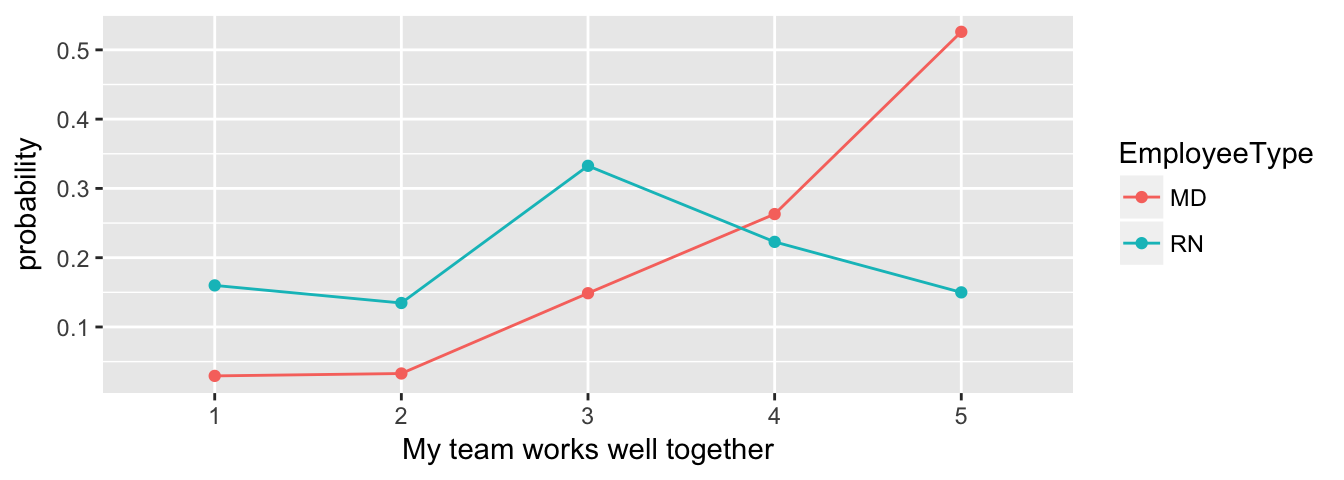
\includegraphics{bookdown-demo_files/figure-latex/prop_odds-1} \end{center}

\begin{tabular}{l|r|r|r|r|r|r|r}
\hline
Modnames & K & AICc & Delta\_AICc & ModelLik & AICcWt & LL & Cum.Wt\\
\hline
Employee Type & 5 & 485.9008 & 0.00000 & 1 & 1 & -237.7686 & 1\\
\hline
Null Model & 4 & 522.0647 & 36.16387 & 0 & 0 & -256.9118 & 1\\
\hline
\end{tabular}

If the concepts or ideas in this section are confusing, it's probably
worth consulting a statistician for help evaluating your data with these
tools.

\hypertarget{Appendix}{\chapter{Appendix: Measurement Levels \&
Appropriate Summary Statistics}\label{Appendix}}

\begin{longtable}[]{@{}lcccc@{}}
\toprule
\begin{minipage}[b]{0.25\columnwidth}\raggedright\strut
Statistic /\\
Parameter\strut
\end{minipage} & \begin{minipage}[b]{0.14\columnwidth}\centering\strut
Categorical\\
\emph{Nominal}\strut
\end{minipage} & \begin{minipage}[b]{0.11\columnwidth}\centering\strut
Ranked\\
\emph{Ordinal}\strut
\end{minipage} & \begin{minipage}[b]{0.18\columnwidth}\centering\strut
Discrete/Counts\\
\emph{Interval/Ratio}\strut
\end{minipage} & \begin{minipage}[b]{0.18\columnwidth}\centering\strut
Continuous\\
\emph{Interval/Ratio}\strut
\end{minipage}\tabularnewline
\midrule
\endhead
\begin{minipage}[t]{0.25\columnwidth}\raggedright\strut
Data set size (n)\\
Percent / Frequency\\
Count or rate\\
Categories (levels)\\
Mode\\
Median\\
Interquartile range\\
Median absolute deviation\\
Range\\
Minimum/maximum value\\
Quantiles\\
Mean (average)\\
Standard deviation\\
Coefficient of variation\\
\strut
\end{minipage} & \begin{minipage}[t]{0.14\columnwidth}\centering\strut
Y\\
Y\\
Y\\
Y\\
Y\\
\emph{No}\\
\emph{No}\\
\emph{No}\\
\emph{No}\\
\emph{No}\\
\emph{No}\\
\emph{No}\\
\emph{No}\\
\emph{No}\\
\strut
\end{minipage} & \begin{minipage}[t]{0.11\columnwidth}\centering\strut
Y\\
Y\\
Y\\
Y\\
Y\\
Y\\
Y\\
Y\\
Y\\
Y\\
Y\\
\emph{No}\\
\emph{No}\\
\emph{No}\\
\strut
\end{minipage} & \begin{minipage}[t]{0.18\columnwidth}\centering\strut
Y\\
Y\\
Y\\
Y\\
Y\\
Y\\
Y\\
Y\\
Y\\
Y\\
Y\\
Y\\
Y*\\
Y*\\
\strut
\end{minipage} & \begin{minipage}[t]{0.18\columnwidth}\centering\strut
Y\\
Y\\
Y\\
Y\\
Y\\
Y\\
Y\\
Y\\
Y\\
Y\\
Y\\
Y\\
Y*\\
Y*\\
\strut
\end{minipage}\tabularnewline
\bottomrule
\end{longtable}

* You must use the correct distribution (proper mean-variance
relationship) to ensure you get the correct standard deviation; most
software defaults to calculating the standard deviation for a
normally-distributed sample, which could be incorrect for certain kinds
of count, rate, or proportion data, for example.


\end{document}
